\chapter{Descriptive Statistics}
\label{chap:ch6}

In software engineering, we constantly deal with data: performance metrics, user behavior patterns, system response times, and code complexity measures. To make sense of this information and extract meaningful insights, we need tools to summarize, organize, and visualize data. Descriptive statistics provides these essential tools, allowing us to understand the characteristics of our data without making inferences about larger populations.

Consider a software development team analyzing the performance of their web application. They collect response times for 1000 user requests and find values ranging from 50 milliseconds to 3.2 seconds. Without proper analysis, this raw data is overwhelming and uninformative. However, by applying descriptive statistics, they can determine that the average response time is 450 milliseconds, that 75\% of requests complete within 600 milliseconds, and that there are a few unusually slow requests that might indicate performance issues.

This chapter introduces the fundamental concepts of descriptive statistics, focusing on measures that help us understand the central tendencies, variability, and distribution patterns in our data. We will explore how these techniques apply specifically to software engineering contexts, from analyzing algorithm performance to understanding user behavior patterns.

\section{Introduction to Descriptive Statistics} \label{sec:ch6sec1}

Sometimes statistical work begins with existing data, such as precipitation records, unemployment rates, or GDP figures, which we then summarize and analyze. In other situations, data must be generated through an experiment or study. For example, to compare two teaching methods in an introductory programming course, an instructor might randomly divide students into two groups, apply a different method to each, and then compare test scores. Random assignment is essential: it ensures that differences between groups are not due to preexisting factors such as aptitude, but rather to the teaching method itself.  

After the data are collected, they are summarized and visualized—for example, by reporting the average score for each group. This process is the essence of \textbf{descriptive statistics}: organising, presenting, and describing data in a meaningful way.  

\subsection*{Population versus Sample}

In statistical analysis, we distinguish between two key concepts:

\begin{definition}[Population]
A \textbf{population} is the complete set of all possible observations or measurements of interest in a particular study. In software engineering contexts, this might include all possible execution times of an algorithm, all user sessions on a website, or all lines of code in a project.
\end{definition}

\begin{definition}[Sample]
A \textbf{sample} is a subset of the population that we actually observe or measure. Due to practical constraints, we often work with samples rather than entire populations.
\end{definition}

In the teaching-method example, the students in the classroom form only a \emph{sample} of the larger \emph{population} of potential learners. Descriptive statistics helps us understand the sample itself, while inferential methods later allow us to use that sample to draw conclusions about the broader population. Inferential statistics lies beyond the scope of this book. We will focus on descriptive statistics in this chapter.


\begin{example} Software Performance Analysis

Consider a web application serving millions of users daily. The \textbf{population} would be the response times for all possible user requests. However, due to computational and storage limitations, we might only collect response times for a \textbf{sample} of 10,000 requests per day. This sample should be representative of the population to draw meaningful conclusions.
\end{example}

\subsection*{Types of Data}

Data can be classified into different types, each requiring different statistical approaches:

\begin{definition}[Qualitative Data]
\textbf{Qualitative data} (also called categorical data) consists of non-numerical information that can be categorized. Examples include programming languages used in a project, user satisfaction ratings (satisfied/neutral/dissatisfied), or bug severity levels (critical/high/medium/low).
\end{definition}

The essential difference between \textbf{qualitative} and \textbf{quantitative} data lies in what they represent and how they are analyzed. Qualitative data refers to categories or attributes that cannot be expressed meaningfully as numbers. Such data are used to classify or label elements, for example, programming language or bug severity. Quantitative data, on the other hand, consists of numerical values that represent counts or measurements, such as response times or number of users. Because these values are numerical, they permit mathematical operations and statistical analysis. Recognizing the distinction between qualitative and quantitative data is fundamental, as it guides the choice of statistical methods and the types of visualizations that are appropriate for analysis.

\begin{definition}[Quantitative Data]
\textbf{Quantitative data} consists of numerical measurements that can be ordered and subjected to mathematical operations. This can be further divided into:
\begin{itemize}
    \item \textbf{Discrete}: Countable values (number of bugs, lines of code, user sessions)
    \item \textbf{Continuous}: Measurable values that can take any value within a range (response times, memory usage, CPU utilization)
\end{itemize}
\end{definition}

\begin{example}
\begin{itemize}
    \item \textbf{Qualitative}: Programming language (Python, Java, C++), deployment environment (development, staging, production)
    \item \textbf{Quantitative Discrete}: Number of commits per day, lines of code, number of test cases
    \item \textbf{Quantitative Continuous}: Response time in milliseconds, memory usage in MB, CPU utilization percentage
\end{itemize}
\end{example}

\subsection*{Outliers and Extreme Data}

In any dataset, most values tend to cluster around a central region, but occasionally, we encounter values that are much higher or lower than the rest. These are called \textbf{outliers} or \textbf{extreme values}. Outliers can arise for many reasons: measurement errors, unusual but valid events, or natural variability in the data.

For example, if most web requests complete in under 400 milliseconds, but one request takes 1200 milliseconds, that 1200ms value is an outlier. Outliers can have a strong influence on summary statistics like the mean, making the data appear more variable or shifting the average away from where most values lie.

It's important to look for outliers when analyzing data, as they can signal interesting phenomena (such as a rare performance bottleneck), data entry mistakes, or the need for further investigation. While there are formal methods to detect outliers, which we will discuss later, often a simple plot or a scan of the sorted data is enough to spot values that "stand out" from the rest.

In practice, understanding the context is key: sometimes outliers are errors to be corrected or removed, but other times they are the most important part of the story.

\section{Describing Data Sets}
When presenting numerical results, clarity and brevity are essential. Tables and graphs are particularly effective, as they allow the reader to quickly grasp the main characteristics of a dataset. Visual and tabular summaries often highlight important aspects such as the overall range, how tightly the values are concentrated, and whether the data appear symmetric or skewed.

\subsection*{Frequency Tables and Graphs} \label{sub:frequency_tables_and_graphs}

The first step in data analysis is often to organize raw data into a frequency distribution, which shows how often each value (or range of values) occurs.

\begin{definition}[Frequency Distribution]
A \textbf{frequency distribution} is a table that shows the frequency (count) of each value or class of values in a dataset. It can be presented as:
\begin{itemize}
    \item \textbf{Absolute frequency}: The actual count of occurrences
    \item \textbf{Relative frequency}: The proportion of total observations
    \item \textbf{Cumulative frequency}: The running total of frequencies
\end{itemize}
\end{definition}

\begin{example}
A dataset with a relatively small number of distinct values can be conveniently presented in a frequency table. For instance, consider a dataset consisting of the starting monthly salaries (to the nearest thousand Danish Kroner) of 42 recently graduated students with B.S. degrees in software engineering.

The raw data is as follows:
\[
\begin{aligned}
&37, 37, 37, 37, 38, 39, 39, 39, 40, 40, 40, 40, 40, 41, 41, 41, 41, 41, 41, 41, 41, \\
&42, 42, 42, 42, 42, 42, 42, 42, 42, 42, 44, 44, 44, 44, 44, 46, 46, 47, 47, 47, 50
\end{aligned}
\]

From this data, we can construct a frequency table. \autoref{tab:salary_freq} tells us, among other things, that the lowest starting salary of 37,000 DKK was received by four of the graduates, whereas the highest salary of 50,000 DKK was received by a single student. The most common starting salary was 42,000 DKK, received by 10 of the students.

\begin{table}[htbp]
\centering
\renewcommand{\arraystretch}{1.2}
{\arrayrulecolor{mseViaBlue}
\begin{tabular}{cc}
\toprule
\textbf{Salary (\(\times 1000\) DKK)} & \textbf{Frequency} \\
\midrule
37 & 4 \\
38 & 1 \\
39 & 3 \\
40 & 5 \\
41 & 8 \\
42 & 10 \\
44 & 5 \\
46 & 2 \\
47 & 3 \\
50 & 1 \\
\bottomrule
\end{tabular}
}
\caption{Frequency Distribution of Monthly Starting Salaries}
\label{tab:salary_freq}
\end{table}
\end{example}

Data from a frequency table can be graphically represented by a line graph that plots the
distinct data values on the horizontal axis and indicates their frequencies by the heights of
vertical lines. A line graph of the data presented in \autoref{tab:salary_freq} is shown in \autoref{fig:salary_line_graph}.

\begin{figure}[htbp]
\centering
\begin{tikzpicture}
\begin{axis}[
    title={Line Graph of Starting Salaries},
    xlabel={Starting Salary (\(\times 1000\) DKK)},
    ylabel={Frequency},
    ymin=0,
    ymax=12,
    xmin=36,
    xmax=51,
    grid=major,
    grid style={dashed,gray!30},
    xtick={37,38,...,50},
    xticklabel style={rotate=45, anchor=east, yshift=-5pt},
    width=0.9\linewidth,
    height=7cm,
    title style={font=\large\bfseries}
]
\addplot+[ycomb, mseViaBlue, thick, mark=*, mark options={fill=mseViaBlue,draw=mseViaBlue}] coordinates {
    (37, 4)
    (38, 1)
    (39, 3)
    (40, 5)
    (41, 8)
    (42, 10)
    (44, 5)
    (46, 2)
    (47, 3)
    (50, 1)
};
\end{axis}
\end{tikzpicture}
\caption{A line graph showing the frequency of different starting salaries.}
\label{fig:salary_line_graph}
\end{figure}

When the lines in a line graph are given added thickness, the graph is called a bar graph. \autoref{fig:salary_bar_graph} shows a bar graph for the same salary data.

\newpage   

\begin{figure}[htbp]
\centering
\begin{tikzpicture}
\begin{axis}[
    title={Bar Graph of Starting Salaries},
    xlabel={Starting Salary (\(\times 1000\) DKK)},
    ylabel={Frequency},
    ymin=0,
    ymax=12,
    xmin=36,
    xmax=51,
    grid=major,
    grid style={dashed,gray!30},
    xtick={37,38,...,50},
    xticklabel style={rotate=45, anchor=east, yshift=-5pt},
    width=0.9\linewidth,
    height=7cm,
    title style={font=\large\bfseries},
    ybar,
    bar width=0.6cm
]
\addplot[fill=mseViaBlue, draw=mseViaBlue!80!black] coordinates {
    (37, 4)
    (38, 1)
    (39, 3)
    (40, 5)
    (41, 8)
    (42, 10)
    (43, 0)
    (44, 5)
    (46, 2)
    (47, 3)
    (50, 1)
};
\end{axis}
\end{tikzpicture}
\caption{A bar graph of the salary data.}
\label{fig:salary_bar_graph}
\end{figure}

Another type of graph used to represent a frequency table is the frequency polygon, which
plots the frequencies of the different data values on the vertical axis, and then connects the
plotted points with straight lines. \autoref{fig:salary_frequency_polygon} shows a frequency polygon for the same salary data.

\begin{figure}[htbp]
\centering
\begin{tikzpicture}
\begin{axis}[
    title={Frequency Polygon of Starting Salaries},
    xlabel={Starting Salary (\(\times 1000\) DKK)},
    ylabel={Frequency},
    ymin=0,
    ymax=12,
    xmin=36,
    xmax=51,
    grid=major,
    grid style={dashed,gray!30},
    xtick={37,38,...,50},
    xticklabel style={rotate=45, anchor=east, yshift=-5pt},
    width=0.9\linewidth,
    height=7cm,
    title style={font=\large\bfseries}
]
\addplot[color=mseViaBlue, thick, mark=*, mark options={fill=mseViaBlue}] coordinates {
    (37, 4)
    (38, 1)
    (39, 3)
    (40, 5)
    (41, 8)
    (42, 10)
    (43, 0)
    (44, 5)
    (45, 0)
    (46, 2)
    (47, 3)
    (48, 0)
    (49, 0)
    (50, 1)
};
\end{axis}
\end{tikzpicture}
\caption{A frequency polygon of the salary data, connecting the points from the frequency table.}
\label{fig:salary_frequency_polygon}
\end{figure}

Sometimes we prefer the relative frequency over the absolute frequency. This is particularly useful when dealing with large datasets and when you want to compare values from datasets of different sizes. An extension of the relative frequency is the cumulative relative frequency, which is the running total of the relative frequencies. \autoref{tab:salary_full_freq} shows the frequency, relative frequency, and cumulative relative frequency for the salary data.

\begin{table}[htbp]
\centering
\renewcommand{\arraystretch}{1.3}
{\arrayrulecolor{mseViaBlue}
\begin{tabular}{cccc}
\toprule
\textbf{Salary} & \textbf{Frequency} & \textbf{Relative Freq.} & \textbf{Cumulative Rel. Freq.} \\
\midrule
37 & 4 & $4/42 \approx 0.095$ & $4/42 \approx 0.095$ \\
38 & 1 & $1/42 \approx 0.024$ & $5/42 \approx 0.119$ \\
39 & 3 & $3/42 \approx 0.071$ & $8/42 \approx 0.190$ \\
40 & 5 & $5/42 \approx 0.119$ & $13/42 \approx 0.310$ \\
41 & 8 & $8/42 \approx 0.190$ & $21/42 = 0.500$ \\
42 & 10 & $10/42 \approx 0.238$ & $31/42 \approx 0.738$ \\
44 & 5 & $5/42 \approx 0.119$ & $36/42 \approx 0.857$ \\
46 & 2 & $2/42 \approx 0.048$ & $38/42 \approx 0.905$ \\
47 & 3 & $3/42 \approx 0.071$ & $41/42 \approx 0.976$ \\
50 & 1 & $1/42 \approx 0.024$ & $42/42 = 1.000$ \\
\bottomrule
\end{tabular}
}
\caption{Frequency, Relative Frequency, and Cumulative Relative Frequency of Monthly Starting Salaries.}
\label{tab:salary_full_freq}
\end{table}

\newpage

\subsection*{Grouped Data and Histograms}

As we saw in \autoref{sub:frequency_tables_and_graphs}, line and bar graphs are useful for showing frequencies of data values. When a dataset contains many distinct values, such as the lamp lifetimes in \autoref{tab:lamp_life_raw}, creating a frequency table for each individual value becomes impractical. A more effective approach is to group the data into a set of \textbf{class intervals}, which are also commonly referred to as \textbf{bins}.

\begin{table}[h!]
\centering
\small % Use a smaller font for the large table
\renewcommand{\arraystretch}{1.2}
{\arrayrulecolor{mseViaBlue}
\begin{tabular}{rrrrrrrrrr}
\toprule
\multicolumn{10}{c}{\textbf{Item Lifetimes (in Hours)}} \\
\midrule
1067 & 919 & 1196 & 785 & 1126 & 936 & 918 & 1156 & 920 & 948 \\
855 & 1092 & 1162 & 1170 & 929 & 950 & 905 & 972 & 1035 & 1045 \\
1157 & 1195 & 1195 & 1340 & 1122 & 938 & 970 & 1237 & 956 & 1102 \\
1022 & 978 & 832 & 1009 & 1157 & 1151 & 1009 & 765 & 958 & 902 \\
923 & 1333 & 811 & 1217 & 1085 & 896 & 958 & 1311 & 1037 & 702 \\
521 & 933 & 928 & 1153 & 946 & 858 & 1071 & 1069 & 830 & 1063 \\
930 & 807 & 954 & 1063 & 1002 & 909 & 1077 & 1021 & 1062 & 1157 \\
999 & 932 & 1035 & 944 & 1049 & 940 & 1122 & 1115 & 833 & 1320 \\
901 & 1324 & 818 & 1250 & 1203 & 1078 & 890 & 1303 & 1011 & 1102 \\
996 & 780 & 900 & 1106 & 704 & 621 & 854 & 1178 & 1138 & 951 \\
1187 & 1067 & 1118 & 1037 & 958 & 760 & 1101 & 949 & 992 & 966 \\
824 & 653 & 980 & 935 & 878 & 934 & 910 & 1058 & 730 & 980 \\
844 & 814 & 1103 & 1000 & 788 & 1143 & 935 & 1069 & 1170 & 1067 \\
1037 & 1151 & 863 & 990 & 1035 & 1112 & 931 & 970 & 932 & 904 \\
1026 & 1147 & 883 & 867 & 990 & 1258 & 1192 & 922 & 1150 & 1091 \\
1039 & 1083 & 1040 & 1289 & 699 & 1083 & 880 & 1029 & 658 & 912 \\
1023 & 984 & 856 & 924 & 801 & 1122 & 1292 & 1116 & 880 & 1173 \\
1134 & 932 & 938 & 1078 & 1180 & 1106 & 1184 & 954 & 824 & 529 \\
998 & 996 & 1133 & 765 & 775 & 1105 & 1081 & 1171 & 705 & 1425 \\
610 & 916 & 1001 & 895 & 709 & 860 & 1110 & 1149 & 972 & 1002 \\
\bottomrule
\end{tabular}
}
\caption{Life in Hours of 200 Incandescent Lamps.}
\label{tab:lamp_life_raw}
\end{table}

The choice of how many bins to use involves a trade-off. If there are too few bins, we risk losing important information by grouping too many distinct values together. If there are too many bins, the frequencies within each bin may become too small to reveal any clear pattern in the data's distribution.

While the optimal number of bins is a subjective choice that depends on the dataset, a selection of 5 to 10 bins is typical. It is also customary, though not required, to use bins of equal width, as this often makes interpretation easier.

The endpoints of a bin are called its \textbf{class boundaries}. We will adopt the common \textbf{left-end inclusion convention}, which specifies that a bin contains its left-end boundary but not its right-end one. For example, the bin 700--800 would contain any value \(x\) such that \(700 \le x < 800\).

Following this approach, the raw data from \autoref{tab:lamp_life_raw} is summarized in \autoref{tab:lamp_life_freq} using bins of length 100, starting at 500.

\begin{table}[htbp]
\centering
\renewcommand{\arraystretch}{1.3}
{\arrayrulecolor{mseViaBlue}
\begin{tabular}{cccc}
\toprule
\textbf{Class Interval} & \textbf{Frequency} & \textbf{Relative Freq.} & \textbf{Cumulative Rel. Freq.} \\
\midrule
500--600   & 2   & 0.010 & 0.010 \\
600--700   & 5   & 0.025 & 0.035 \\
700--800   & 12  & 0.060 & 0.095 \\
800--900   & 25  & 0.125 & 0.220 \\
900--1000  & 58  & 0.290 & 0.510 \\
1000--1100 & 41  & 0.205 & 0.715 \\
1100--1200 & 43  & 0.215 & 0.930 \\
1200--1300 & 7   & 0.035 & 0.965 \\
1300--1400 & 6   & 0.030 & 0.995 \\
1400--1500 & 1   & 0.005 & 1.000 \\
\bottomrule
\end{tabular}
}
\caption{Frequency Distribution for the Lifetimes of 200 Incandescent Lamps.}
\label{tab:lamp_life_freq}
\end{table}

A bar graph that plots the frequencies of data grouped into bins is called a \textbf{histogram}. A key feature of a histogram is that the bars are placed directly adjacent to one another, reflecting the continuous nature of the bins. The vertical axis can represent either the absolute frequency (the count of values in each interval) or the relative frequency. The former is called a \textbf{frequency histogram}, while the latter is a \textbf{relative frequency histogram}. \autoref{fig:lamp_life_histogram} shows a frequency histogram for the lamp lifetime data.

\newpage

\begin{figure}[htbp]
\centering
\begin{tikzpicture}
\begin{axis}[
    title={Frequency Histogram of Lamp Lifetimes},
    xlabel={Lifetime (in Hours)},
    ylabel={Frequency},
    ymin=0,
    width=0.9\linewidth,
    height=7cm,
    ybar interval,
    xticklabel={\pgfmathprintnumber\tick--\pgfmathprintnumber\nexttick},
    xticklabel style={rotate=45, anchor=east, yshift=-5pt},
    grid=major,
    grid style={dashed,gray!30},
    title style={font=\large\bfseries}
]
\addplot[fill=mseViaBlue, draw=mseViaBlue!80!black] coordinates {
    (500, 2)
    (600, 5)
    (700, 12)
    (800, 25)
    (900, 58)
    (1000, 41)
    (1100, 43)
    (1200, 7)
    (1300, 6)
    (1400, 1)
    (1500, 0)
};
\end{axis}
\end{tikzpicture}
\caption{A frequency histogram for the lamp lifetime data. The adjacent bars show the distribution of data across continuous intervals.}
\label{fig:lamp_life_histogram}
\end{figure}

Finally, we are sometimes interested in plotting the cumulative frequency or, more commonly, the cumulative relative frequency. Such a graph, often called an \textbf{ogive}, shows the number or proportion of data points that fall at or below a certain value.

\begin{figure}[h!]
\centering
\begin{tikzpicture}
\begin{axis}[
    title={Cumulative Relative Frequency of Lamp Lifetimes (Ogive)},
    xlabel={Lifetime (in Hours)},
    ylabel={Cumulative Relative Frequency},
    ymin=0, ymax=1.05,
    xmin=400, xmax=1500,
    width=0.9\linewidth,
    height=7cm,
    grid=major,
    grid style={dashed,gray!30},
    title style={font=\large\bfseries}
]
\addplot[color=mseViaBlue, thick, mark=*, mark options={fill=mseViaBlue}] coordinates {
    (500, 0)
    (600, 0.010)
    (700, 0.035)
    (800, 0.095)
    (900, 0.220)
    (1000, 0.510)
    (1100, 0.715)
    (1200, 0.930)
    (1300, 0.965)
    (1400, 0.995)
    (1500, 1.000)
};
\end{axis}
\end{tikzpicture}
\caption{An ogive showing the cumulative relative frequency for the lamp lifetime data.}
\label{fig:lamp_life_ogive}
\end{figure}

On an ogive, each point on the horizontal axis represents a data value, while the corresponding point on the vertical axis shows the proportion of the data that is less than or equal to that value. For example, \autoref{fig:lamp_life_ogive} presents the cumulative relative frequency plot for the lamp lifetime data. From this graph, we can quickly determine that approximately 50\% of the lamps had a lifetime of less than 1000 hours, about 95\% had a lifetime of less than 1200 hours (the actual value is 93\%), and 100\% of the lamps failed by 1500 hours.

\section{Summarizing Data}
Having seen how to visually and numerically summarize data distributions, we now focus on two fundamental aspects of describing a dataset: its \emph{center} (or typical value) and its \emph{dispersion} (or variability).

\subsection*{Measures of Central Tendency}
The \textbf{mean}, often called the average, is the most commonly used measure of central tendency. \autoref{def:arithmetic_mean} shows how to calculate the mean of a dataset and \autoref{ex:mean_response_time} examplifies .

\begin{definition}[Arithmetic Mean] \label{def:arithmetic_mean}

For a dataset with $n$ values $x_1, x_2, \ldots, x_n$, the \textbf{arithmetic mean} is defined as:

$$
\bar{x} = \frac{1}{n}\sum_{i=1}^{n} x_i = \frac{x_1 + x_2 + \cdots + x_n}{n}
$$

\end{definition}


\begin{example} Response Time Analysis \label{ex:mean_response_time}

A web application recorded the following response times (in milliseconds) for 10 requests:

\[
\{120, 150, 180, 200, 220, 250, 280, 300, 350, 400\}
\]

The mean response time is:
\[
\bar{x} = \frac{120 + 150 + 180 + 200 + 220 + 250 + 280 + 300 + 350 + 400}{10} = \frac{2450}{10} = 245 \text{ milliseconds}
\]
\end{example}

The mean incorporates every value in a dataset, which makes it a powerful measure of central tendency. It is most appropriate when the data values are of similar magnitude and when the distribution is reasonably symmetric without extreme outliers. Under these conditions, the mean provides a reliable summary of the dataset.

For example, in the analysis of web performance, the mean response time offers an overall indication of how quickly a system responds on average. However, if a few response times are much slower than the rest, the mean may give a misleading impression of the typical user experience.

Beyond its role as a summary statistic, the mean also serves as a foundation for many statistical methods. In particular, it is central to the definitions of variance and standard deviation, which measure the dispersion of data around the mean.

\begin{remark}
    As mentioned earlier, and as we will revisit, the mean is highly sensitive to extreme values or outliers. Even a single unusually large or small observation can shift the mean considerably, reducing its ability to reflect the typical value of the dataset.
    It is therefore important to consider the distribution of the data before relying solely on the mean to describe the center of a dataset.
\end{remark}

The \textbf{median} is the middle value when data is arranged in ascending order. It is less sensitive to outliers than the mean.

\begin{definition}[Median]
    For a dataset with $n$ values arranged in ascending order, the median is defined as:
    \[
    \text{median} =
    \begin{cases}
        x_{\frac{n+1}{2}} & \text{if } n \text{ is odd} \\
        \frac{x_{\frac{n}{2}} + x_{\frac{n}{2}+1}}{2} & \text{if } n \text{ is even}
    \end{cases}
    \]
\end{definition}

\begin{example} Median Response Time

Using the same response time data from the previous example:
\[
\{120, 150, 180, 200, 220, 250, 280, 300, 350, 400\}
\]

Since $n = 10$ (even), the median is the average of the 5th and 6th values:
\[
\text{Median} = \frac{220 + 250}{2} = 235 \text{ milliseconds}
\]
\end{example}

\begin{example}

Consider the same data with an extreme value:
\[
\{120, 150, 180, 200, 220, 250, 280, 300, 350, 2000\}
\]

The mean becomes: $\bar{x} = \frac{4050}{10} = 405$ milliseconds (significantly affected by the outlier)

The median remains: $\frac{220 + 250}{2} = 235$ milliseconds (unaffected by the outlier)
\end{example}

Because the median divides a dataset into two equal halves, it serves as a robust measure of central tendency, particularly when the data contain outliers or are skewed. Unlike the mean, which can be drawn toward extreme values, the median remains largely unaffected, offering a more reliable indication of the ``typical'' value in such situations.

The \textbf{mode} is the most frequently occurring value in a dataset.

\begin{definition}[Mode]
The \textbf{mode} is the value that appears most frequently in a dataset. A dataset can have:
\begin{itemize}
    \item \textbf{No mode}: If all values appear with equal frequency
    \item \textbf{One mode (unimodal)}: If one value appears most frequently
    \item \textbf{Multiple modes (multimodal)}: If two or more values tie for the highest frequency
\end{itemize}
\end{definition}

Sometimes, when a data set has two modes, it is called a \textbf{bimodal} dataset.

\newpage

\begin{example}

A software project has the following bug severity levels:
\[
\{\text{High}, \text{Medium}, \text{Low}, \text{High}, \text{Critical}, \text{Medium}, \text{High}, \text{Low}, \text{High}, \text{Medium}\}
\]

Counting frequencies:
\begin{itemize}
    \item High: 4 occurrences
    \item Medium: 3 occurrences  
    \item Low: 2 occurrences
    \item Critical: 1 occurrence
\end{itemize}

The mode is "High" since it appears most frequently.
\end{example}

The mode is especially useful when analyzing categorical or discrete data, where calculating a mean or median may not make sense. For example, in software engineering, the mode can help identify the most common error code returned by an API, the most frequently used programming language in a codebase, or the most reported type of bug in an issue tracker.

\subsubsection*{When to Use Each Measure}

\begin{table}[htbp]
\centering
\renewcommand{\arraystretch}{1.4}
\begin{tabular}{|l|l|l|}
\hline
\textbf{Measure} & \textbf{Best For} & \textbf{Limitations} \\
\hline
Mean & Continuous data, symmetric distributions & Sensitive to outliers \\
\hline
Median & Data with outliers, skewed distributions & Less informative for symmetric data \\
\hline
Mode & Categorical data, discrete data & May not exist or be unique \\
\hline
\end{tabular}
\caption{Comparison of Central Tendency Measures}
\label{tab:central_tendency}
\end{table}

\subsection*{Measures of Dispersion}

While measures of central tendency tell us about the typical value, \textbf{measures of dispersion} describe how spread out the data are.Understanding variability is crucial in software engineering for assessing consistency and reliability.

The \textbf{range} is the simplest measure of dispersion.

\begin{definition}[Range]
The \textbf{range} of a dataset is the difference between the maximum and minimum values:
\[
\text{Range} = x_{\max} - x_{\min}
\]
\end{definition}

\begin{example}

    For the response time data: $\{120, 150, 180, 200, 220, 250, 280, 300, 350, 400\}$

\[
\text{Range} = 400 - 120 = 280 \text{ milliseconds}
\]
\end{example}

\begin{remark}
The range is sensitive to outliers and doesn't provide information about the distribution of values between the extremes.
\end{remark}

The \textbf{variance} and \textbf{standard deviation} are more sophisticated measures that consider all data points.

\begin{definition}[Sample Variance and Standard Deviation]
For a sample with $n$ values, the \textbf{sample variance}, denoted by $s^2$, is defined as:
$$
s^2 = \frac{1}{n-1}\sum_{i=1}^{n}(x_i - \bar{x})^2
$$
The \textbf{sample standard deviation}, denoted by $s$, is the square root of the variance:
$$
s = \sqrt{s^2} = \sqrt{\frac{1}{n-1}\sum_{i=1}^{n}(x_i - \bar{x})^2}
$$
\end{definition}

While the mean identifies the center of a dataset, the \textbf{variance} and \textbf{standard deviation} measure its variability or spread. A small standard deviation indicates that data points are clustered tightly around the mean, whereas a large standard deviation signifies that they are more spread out.

The variance is the average of the squared deviations from the mean. Squaring each deviation serves two purposes: it ensures all values are positive, and it gives greater weight to larger, more significant deviations. However, this calculation leaves the variance in squared units (e.g., milliseconds squared), which are not intuitive to interpret.

To solve this, we use the standard deviation, which is simply the square root of the variance. This crucial step returns the measure to the original units of the data (e.g., milliseconds), making it directly interpretable. In short, the standard deviation represents the typical distance of a data point from the mean.

\begin{example} Calculating Standard Deviation

    For the response time data: $\{120, 150, 180, 200, 220, 250, 280, 300, 350, 400\}$ with $\bar{x} = 245$:

\begin{align*}
s^2 &= \frac{1}{9}[(120-245)^2 + (150-245)^2 + \cdots + (400-245)^2] \\
&= \frac{1}{9}[(-125)^2 + (-95)^2 + \cdots + (155)^2] \\
&= \frac{1}{9}[15625 + 9025 + \cdots + 24025] \\
&= \frac{1}{9} \times 82250 \approx 9138.89
\end{align*}

\[
s = \sqrt{9138.89} \approx 95.6 \text{ milliseconds}
\]
\end{example}

The following algebraic identity is often helpful when computing variance or standard deviation by hand:

We start from the definition:

\[
s^2 = \frac{1}{n-1}\sum_{i=1}^n (x_i - \bar{x})^2
\]

Using the identity

\[
\sum_{i=1}^n (x_i - \bar{x})^2 = \sum_{i=1}^n x_i^2 - \frac{\left(\sum_{i=1}^n x_i \right)^2}{n}
\]

we can rewrite sample variance as

\[
s^2 = \frac{1}{n-1} \left( \sum_{i=1}^n x_i^2 - \frac{\left(\sum_{i=1}^n x_i\right)^2}{n} \right) =\frac{1}{n-1}\left(\sum_{i=1}^n x_i^2-n \bar{x}^2\right)
\]

This is known as the \textbf{computational formula for variance}, as it allows you to calculate $s^2$ directly from $\sum x_i$ and $\sum x_i^2$ (or equivalently, from $\sum x_i^2$ and $\bar{x}$), without needing to compute each individual deviation from the mean.


The \textbf{coefficient of variation} allows comparison of variability across datasets with different scales.

\begin{definition}[Coefficient of Variation]
The \textbf{coefficient of variation} is the ratio of standard deviation to the mean:
\[
CV = \frac{s}{\bar{x}} \times 100\%
\]
\end{definition}

\begin{example} Comparing Variability

Consider two systems:
\begin{itemize}
    \item System A: Mean response time = 100ms, Standard deviation = 20ms
    \item System B: Mean response time = 500ms, Standard deviation = 100ms
\end{itemize}

\begin{align*}
CV_A &= \frac{20}{100} \times 100\% = 20\% \\
CV_B &= \frac{100}{500} \times 100\% = 20\%
\end{align*}

Both systems have the same relative variability (20\%), despite different absolute standard deviations.
\end{example}

\subsection*{Measures of Position}

To introduce a measure of spread that is less sensitive to outliers, we first need to understand measures of position, which describe the relative standing of a data point within a dataset.

\begin{definition}[Percentile]
The $p$-th \textbf{percentile} is the value below which $p\%$ of the data falls.
\end{definition}

For example, if a response time is at the 95th percentile, it means that 95\% of all response times are faster than this one.

\begin{example} Percentile Calculation

    For the response time data, to find the 90th percentile:
\begin{enumerate}
        \item Sort data: $\{120, 150, 180, 200, 220, 250, 280, 300, 350, 400\}$
        \item Position: $0.9 \times 10 = 9$th position
        \item 90th percentile = 350ms
\end{enumerate}
    \end{example}

Quartiles are specific, widely used percentiles that divide the data into four equal parts.

\begin{definition}[Quartiles]

Quartiles divide an ordered dataset into four equal parts.

\begin{itemize}
    \item \textbf{Q1 (First Quartile)}: The 25th percentile. 25\% of the data is less than this value.
    \item \textbf{Q2 (Second Quartile)}: The 50th percentile. This is the \textbf{median} of the dataset.
    \item \textbf{Q3 (Third Quartile)}: The 75th percentile. 75\% of the data is less than this value.
    \item \textbf{Q4 (Fourth Quartile)}: The 100th percentile. 100\% of the data is less than this value.
\end{itemize}
\end{definition}

\begin{example} Calculating Quartiles

For the sorted response time data: $\{120, 150, 180, 200, 220, | 250, 280, 300, 350, 400\}$
\begin{itemize}
    \item The lower half is $\{120, 150, 180, 200, 220\}$. The median of this half is $Q1 = 180$~ms.
    \item The upper half is $\{250, 280, 300, 350, 400\}$. The median of this half is $Q3 = 300$~ms.
\end{itemize}
\end{example}

Percentiles divide data into 100 equal parts, while quartiles divide data into four equal parts.

The \textbf{interquartile range} is a robust measure of dispersion that is not affected by outliers.

\begin{definition}[Interquartile Range]
    The \textbf{interquartile range (IQR)} measures the spread of the middle 50\% of the data and is defined as
    $$
    IQR = Q_3 - Q_1,
    $$
    where $Q_1$ and $Q_3$ are the first and third quartiles. A larger IQR indicates that the central portion of the data is more widely dispersed, while a smaller IQR indicates that it is more tightly clustered.
\end{definition}
    

\begin{example} IQR Calculation

For the response time data: $\{120, 150, 180, 200, 220, 250, 280, 300, 350, 400\}$

\begin{itemize}
    \item Lower half: $\{120, 150, 180, 200, 220\}$ → $Q1 = 180$
    \item Upper half: $\{250, 280, 300, 350, 400\}$ → $Q3 = 300$
    \item $IQR = 300 - 180 = 120$ milliseconds
\end{itemize}
\end{example}


\subsection*{Summary Statistics}

Before we conclude this chapter, we will review the summary statistics that we have covered in this section. Let us consider the response time data again, but now in the form of a table of 1000 values. \autoref{tab:summary_stats} shows the complete statistical summary of the data.

\begin{example}

For a dataset of 1000 web response times:

\begin{table}[htbp]
\centering
\renewcommand{\arraystretch}{1.3}
\begin{tabular}{|l|c|}
\hline
\textbf{Measure} & \textbf{Value} \\
\hline
Count & 1000 \\
Mean & 245.3 ms \\
Median & 238.0 ms \\
Mode & 220.0 ms \\
Standard Deviation & 95.6 ms \\
Variance & 9138.9 ms² \\
Minimum & 45.0 ms \\
Maximum & 1200.0 ms \\
Range & 1155.0 ms \\
Q1 & 180.0 ms \\
Q3 & 300.0 ms \\
IQR & 120.0 ms \\
Skewness & 1.2 (positive skew) \\
Kurtosis & 2.8 (leptokurtic) \\
\hline
\end{tabular}
\caption{Complete Statistical Summary}
\label{tab:summary_stats}
\end{table}
\end{example}

This table provides a complete picture of the data and is often a first step in the analysis of a dataset. Note that the skewness and kurtosis have not been discussed but will be explained in the next section. We have chosen to include them here for completeness as they are often used in the analysis of a dataset - although how to calculate them is beyond the scope of this book.


\section{Understanding Data Distributions} \label{sec:data_distributions}
Once we have visualized our data with histograms and box plots, we can begin to analyze the \textit{shape} of the distribution. The shape tells us about the underlying patterns in our data and helps us choose the right statistical tools. In software engineering, understanding the distribution of metrics like response times or error rates is critical for setting performance baselines and detecting anomalies. First we review the concept of outliers.

\subsection*{Normal Data Sets}

Many large data sets yield histograms with a distinctive overall shape: the frequencies peak near the sample median and decrease symmetrically on both sides, forming a characteristic \textbf{bell-shaped curve}. Data sets exhibiting this property are called \textbf{normal}, and their histograms are referred to as \textbf{normal histograms} (see \autoref{fig:normal_hist}).

\begin{figure}[htbp]
    \centering
    \begin{tikzpicture}
    \begin{axis}[
        width=0.6\textwidth,
        height=6cm,
        ybar,
        bar width=1,
        enlargelimits=0.05,
        ylabel={Frequency},
        xmin=1.1,
        xmax=18,
        xtick=\empty,
        ytick=\empty,
        axis lines*=left,
        y axis line style={opacity=1},
        x axis line style={opacity=1},
        grid=major, 
        grid style={dashed,gray!30}, 
        xmajorgrids=false,
        ]
    \addplot[fill=mseViaBlue, draw=mseViaBlue!80!black] coordinates {
        (1, 1) (2, 2) (3, 4) (4, 7) (5, 9) (6, 11) (7, 13) (8, 15) (9, 17) (10, 15) (11, 13) (12, 11) (13, 9) (14, 7) (15, 4) (16, 2) (17, 1)
    };
    \end{axis}
    \end{tikzpicture}
    \caption{A histogram of a normal data set, showing the characteristic bell shape.}
    \label{fig:normal_hist}
\end{figure}


In software systems, perfectly normal distributions are rare, but some metrics can be \textbf{approximately normal}. For example, the latency of a highly optimized, internal microservice that performs a consistent task might be approximately normal. A histogram of an approximately normal data set looks like \autoref{fig:approx_normal_hist}.

\begin{figure}[htbp]
    \centering
    \begin{tikzpicture}
    \begin{axis}[
        width=0.6\textwidth,
        height=6cm,
        ybar,
        bar width=1,
        enlargelimits=0.05,
        ylabel={Frequency},
        xmin=1.1,
        xmax=18,
        xtick=\empty,
        ytick=\empty,
        axis lines*=left,
        y axis line style={opacity=1},
        x axis line style={opacity=1},
        grid=major, 
        grid style={dashed,gray!30}, 
        xmajorgrids=false,
        ]
    \addplot[fill=mseViaBlue, draw=mseViaBlue!80!black] coordinates {
        (1,1) (2,2) (3,3) (4,5) (5,7) (6,9) (7,11) (8,12) (9,10) (10,11) (11,9) (12,7) (13,4) (14,2) (15,1) (17,2)
    };
    \end{axis}
    \end{tikzpicture}
    \caption{A histogram of a data set that is approximately normal. While not perfectly symmetric, it follows the general bell shape.}
    \label{fig:approx_normal_hist}
\end{figure}

Many datasets observed in practice, from human height to measurement errors, follow this specific shape. Such data is said to be \textbf{normally distributed}.

\begin{definition}[Normal Distribution]
A \textbf{normal distribution} is a symmetric, bell-shaped distribution where the mean, median, and mode are all equal and located at the center. Its shape is determined entirely by its mean ($\mu$) and standard deviation ($\sigma$).
\end{definition}

When the bins of a histogram become smaller, the histogram becomes more and more similar to a normal distribution. This is because the normal distribution is a continuous distribution, while the histogram is a discrete distribution. This is a consequence of the \textbf{Law of Large Numbers}.

\begin{theorem}[Law of Large Numbers]
    The sample mean of a dataset will converge to the population mean as the sample size increases.
\end{theorem}

When the sample size is large enough, the sample mean will be very close to the population mean, and the histogram will be very similar to a normal distribution and will get the following shape:

\begin{figure}[htbp]
    \centering
    \begin{tikzpicture}
    \begin{axis}[
        width=0.6\textwidth,
        height=6cm,
        axis lines*=left,
        xmin=0,
        xmax=10,
        ymin=0,
        ymax=0.5,
        xtick=\empty,
        ytick=\empty,
        grid=major,
        grid style={dashed,gray!30},
        xmajorgrids=false
    ]
    % Smooth normal curve (mean at 5, sd ~1.3) in mseViaBlue
    \addplot[smooth, very thick, color=mseViaBlue, samples=200, domain=0:10] { 0.45*exp(-0.5*((x-5)/1.3)^2) };
    \end{axis}
    \end{tikzpicture}
    \caption{The normal distribution curve.}
    \label{fig:normal_curve_smooth}
\end{figure}

For data that is approximately normal, we can use a powerful rule of thumb to understand its spread without looking at every single data point. This is known as the \textbf{Empirical Rule}.

\begin{theorem}[The Empirical Rule]
If a dataset is approximately normal with a sample mean $\bar{x}$ and sample standard deviation $s$, then:
\begin{itemize}
    \item Approximately \textbf{68.3\%} of the observations lie within 1 standard deviation of the mean ($\bar{x} \pm s$).
    \item Approximately \textbf{95.4\%} of the observations lie within 2 standard deviations of the mean ($\bar{x} \pm 2s$).
    \item Approximately \textbf{99.7\%} of the observations lie within 3 standard deviations of the mean ($\bar{x} \pm 3s$).
\end{itemize}
\end{theorem}

\begin{figure}[htbp]
    \centering
    \begin{tikzpicture}
    \begin{axis}[
        width=0.6\textwidth,
        height=6cm,
        axis lines*=left,
        xmin=-3.5,
        xmax=3.5,
        ymin=0,
        ymax=0.5,
        xtick={-3,-2,-1,0,1,2,3},
        ytick=\empty,
        grid=major,
        grid style={dashed,gray!30},
        xmajorgrids=false,
        clip=false
    ]
    % Base light fill (-3σ..+3σ)
    \addplot[domain=-3:3, samples=200, draw=none, fill=mseViaBlue!15] { 0.45*exp(-0.5*(x^2)) } -- (axis cs:3,0) -- (axis cs:-3,0) -- cycle;
    % Medium fill (-2σ..+2σ)
    \addplot[domain=-2:2, samples=200, draw=none, fill=mseViaBlue!30] { 0.45*exp(-0.5*(x^2)) } -- (axis cs:2,0) -- (axis cs:-2,0) -- cycle;
    % Darker fill (-1σ..+1σ)
    \addplot[domain=-1:1, samples=200, draw=none, fill=mseViaBlue!50] { 0.45*exp(-0.5*(x^2)) } -- (axis cs:1,0) -- (axis cs:-1,0) -- cycle;
    % Normal curve outline
    \addplot[smooth, very thick, color=mseViaBlue, samples=200, domain=-3.2:3.2] { 0.45*exp(-0.5*(x^2)) };
    % Vertical sigma lines (calculated to match the curve: 0.45*exp(-0.5*x^2))
    \addplot[mseViaBlue!80!black, thick] coordinates {(-3,0) (-3,0.0050)};
    \addplot[mseViaBlue!80!black, thick] coordinates {(-2,0) (-2,0.0609)};
    \addplot[mseViaBlue!80!black, thick] coordinates {(-1,0) (-1,0.2729)};
    \addplot[mseViaBlue!80!black, thick, dashed] coordinates {(0,0) (0,0.45)};
    \addplot[mseViaBlue!80!black, thick] coordinates {(1,0) (1,0.2729)};
    \addplot[mseViaBlue!80!black, thick] coordinates {(2,0) (2,0.0609)};
    \addplot[mseViaBlue!80!black, thick] coordinates {(3,0) (3,0.0050)};
    % Percentage labels above segments
    \node[font=\scriptsize] at (axis cs:-3.2,0.03) {0.15\%};
    \node[font=\scriptsize] at (axis cs:3.2,0.03) {0.15\%};
    \node[font=\scriptsize] at (axis cs:-2.5,0.08) {2.1\%};
    \node[font=\scriptsize] at (axis cs:2.5,0.08) {2.1\%};
    \node[font=\scriptsize] at (axis cs:-1.5,0.20) {13.6\%};
    \node[font=\scriptsize] at (axis cs:1.5,0.20) {13.6\%};
    \node[font=\scriptsize] at (axis cs:-0.5,0.28) {34.15\%};
    \node[font=\scriptsize] at (axis cs:0.5,0.28) {34.15\%};
    % Braces for 68.3%, 95.4%, 99.7%
    \draw[mseViaBlue!80!black, thick, decorate, decoration={brace, amplitude=4pt, mirror}] (axis cs:-1,-0.05) -- (axis cs:1,-0.05) node[midway, below=4pt, xshift=2pt, font=\scriptsize]{68.3\%};
    \draw[mseViaBlue!80!black, thick, decorate, decoration={brace, amplitude=4pt, mirror}] (axis cs:-2,-0.11) -- (axis cs:2,-0.10) node[midway, below=4pt, xshift=2pt, font=\scriptsize]{95.4\%};
    \draw[mseViaBlue!80!black, thick, decorate, decoration={brace, amplitude=4pt, mirror}] (axis cs:-3,-0.17) -- (axis cs:3,-0.16) node[midway, below=4pt, xshift=2pt, font=\scriptsize]{99.7\%};
    \end{axis}
    \end{tikzpicture}
    \caption{Empirical Rule on a normal curve. The inner bands mark $\pm1\sigma$ (68.3\%), $\pm2\sigma$ (95.4\%), and $\pm3\sigma$ (99.7\%).}
    \label{fig:empirical_rule_shaded}
\end{figure}

\subsection*{Skewed Data Sets}
When a data set is not symmetric about its sample median, it is described as \textbf{skewed}. A long tail extending to the right indicates the distribution is \textbf{skewed to the right}; a long tail to the left means it is \textbf{skewed to the left}. Thus, the histogram in \autoref{fig:left_skewed_hist} is skewed left, while the one in \autoref{fig:right_skewed_hist} is skewed right.

\begin{definition}[Skewness]
    \textbf{Skewness} measures the asymmetry of data distribution:
    \begin{itemize}
        \item \textbf{Positive skew (skewed to the right)}: Tail extends to the right (mean > median)
        \item \textbf{Negative skew (skewed to the left)}: Tail extends to the left (mean < median)
        \item \textbf{Symmetric}: Mean $\approx$ median
    \end{itemize}
    \end{definition}

\begin{figure}[htbp]
    \centering
    \begin{tikzpicture}
        \begin{axis}[
            width=0.6\textwidth,
            height=6cm,
            ybar,
            bar width=1,
            enlargelimits=0.05,
            ylabel={Frequency},
            xmin=1.1,
            xmax=18,
            xtick=\empty,
            ytick=\empty,
            axis lines*=left,
            y axis line style={opacity=1},
            x axis line style={opacity=1},
            grid=major, 
            grid style={dashed,gray!30}, 
            xmajorgrids=false,
            ]
        \addplot[fill=mseViaBlue, draw=mseViaBlue!80!black] coordinates {
            (1, 1) (2, 1) (4, 2) (5, 3) (6, 4) (7, 6) (8, 8) (9, 12) (10, 15) (11, 17) (12, 16) (13, 13) (14, 9) (15, 5) (16,1)
        };
        \end{axis}
    \end{tikzpicture}
    \caption{A histogram of a data set that is skewed to the left (negatively skewed). The tail of the distribution is on the left.}
    \label{fig:left_skewed_hist}
\end{figure}

\begin{figure}[htbp]
    \centering
    \begin{tikzpicture}
        \begin{axis}[
            width=0.6\textwidth,
            height=6cm,
            ybar,
            bar width=1,
            enlargelimits=0.05,
            ylabel={Frequency},
            xmin=1.1,
            xmax=18,
            xtick=\empty,
            ytick=\empty,
            axis lines*=left,
            y axis line style={opacity=1},
            x axis line style={opacity=1},
            grid=major, 
            grid style={dashed,gray!30}, 
            xmajorgrids=false,
            ]
        \addplot[fill=mseViaBlue, draw=mseViaBlue!80!black] coordinates {
            (1, 1) (2, 5) (3, 9) (4, 13) (5, 16) (6, 17) (7, 15) (8, 12) (9, 8) (10, 6) (11, 4) (12, 3) (13, 2) (14, 1) (16, 1)
        };
        \end{axis}
    \end{tikzpicture}
    \caption{A histogram of a data set that is skewed to the right (positively skewed). The tail of the distribution is on the right.}
    \label{fig:right_skewed_hist}
\end{figure}

\newpage

\autoref{fig:skew_mean_median_mode} shows the relationship between mean, median, and mode for right skewed, symmetric, and left skewed distributions.


\begin{figure}[htbp]
    \centering
    % Positive skew panel
    \begin{minipage}{0.32\textwidth}
        \centering
        \begin{tikzpicture}
        \begin{axis}[
            width=\linewidth,
            height=4cm,
            xmin=0, xmax=10,
            ymin=0, ymax=0.5,
            axis lines*=left,
            xtick=\empty,
            ytick=\empty,
            clip=false
        ]
        % Right-tailed (positive skew) smooth curve
        \addplot[smooth, very thick, color=mseViaBlue, samples=200, domain=0:10] { (x)*exp(-0.6*x)/3 };
        % Mode, Median, Mean
        \addplot[mseViaBlue!80!black, thick, dotted] coordinates {(1.7,0) (1.7,0.46)};
        \addplot[third, thick] coordinates {(2.3,0) (2.3,0.46)};
        \addplot[mseViaBlue!80!black, thick, dashed] coordinates {(2.9,0) (2.9,0.46)};
        % Vertical labels (rotated 90 degrees left)
        \node[anchor=west, font=\scriptsize, rotate=45] at (axis cs:1,0.46) {Mode};
        \node[anchor=west, font=\scriptsize, rotate=45] at (axis cs:2,0.46) {Median};
        \node[anchor=west, font=\scriptsize, rotate=45] at (axis cs:3,0.46) {Mean};
        \end{axis}
        \end{tikzpicture}
        \par\small Right Skew
    \end{minipage}
    \hfill
    % Symmetric (normal) panel
    \begin{minipage}{0.32\textwidth}
        \centering
        \begin{tikzpicture}
        \begin{axis}[
            width=\linewidth,
            height=4cm,
            xmin=0, xmax=10,
            ymin=0, ymax=0.5,
            axis lines*=left,
            xtick=\empty,
            ytick=\empty,
            clip=false
        ]
        \addplot[smooth, very thick, color=mseViaBlue, samples=200, domain=0:10] { 0.45*exp(-0.5*((x-5)/1.3)^2) };
        \addplot[mseViaBlue!80!black, thick, dashed] coordinates {(5,0) (5,0.46)};
        \node[anchor=south, font=\scriptsize, align=center] at (axis cs:5,0.48) {Mean\\Median\\Mode};
        \end{axis}
        \end{tikzpicture}
        \par\small Symmetric
    \end{minipage}
    \hfill
    % Negative skew panel
    \begin{minipage}{0.32\textwidth}
        \centering
        \begin{tikzpicture}
        \begin{axis}[
            width=\linewidth,
            height=4cm,
            xmin=0, xmax=10,
            ymin=0, ymax=0.5,
            axis lines*=left,
            xtick=\empty,
            ytick=\empty,
            clip=false
        ]
        % Left-tailed (negative skew) smooth curve
        \addplot[smooth, very thick, color=mseViaBlue, samples=200, domain=0:10] { ((10-x))*exp(-0.6*(10-x))/3 };
        % Mean, Median, Mode (mean left, median middle, mode right)
        \addplot[mseViaBlue!80!black, thick, dashed] coordinates {(7.1,0) (7.1,0.46)};
        \addplot[third, thick] coordinates {(7.7,0) (7.7,0.46)};
        \addplot[mseViaBlue!80!black, thick, dotted] coordinates {(8.3,0) (8.3,0.46)};
        % Vertical labels (rotated 90 degrees left)
        \node[anchor=west, font=\scriptsize, rotate=45] at (axis cs:6.5,0.46) {Mean};
        \node[anchor=west, font=\scriptsize, rotate=45] at (axis cs:7.5,0.46) {Median};
        \node[anchor=west, font=\scriptsize, rotate=45] at (axis cs:8.5,0.46) {Mode};
        \end{axis}
        \end{tikzpicture}
        \par\small Left Skew
    \end{minipage}
    \caption{Relationship between mean, median, and mode for positively skewed, symmetric, and negatively skewed distributions.}
    \label{fig:skew_mean_median_mode}
\end{figure}

\subsection*{Outlier Detection}

As mentioned in \autoref{sec:ch6sec1}, outliers are data points that are significantly different from the rest of the data. They can arise due to measurement errors, data entry errors, or genuine variability in the data. Detecting outliers is important because they can distort statistical analyses.

A common method for identifying outliers is to use the interquartile range (IQR):

\begin{itemize}
    \item \textbf{Mild outliers}: Any data point less than $Q_1 - 1.5 \times IQR$ or greater than $Q_3 + 1.5 \times IQR$.
    \item \textbf{Extreme outliers}: Any data point less than $Q_1 - 3 \times IQR$ or greater than $Q_3 + 3 \times IQR$.
\end{itemize}

\begin{example} Detecting Outliers

Given the response time data: $\{120, 150, 180, 200, 220, 250, 280, 300, 350, 400\}$

\begin{itemize}
    \item $Q_1 = 180$, $Q_3 = 300$, $IQR = 120$
    \item Lower fence: $Q_1 - 1.5 \times IQR = 180 - 180 = 0$
    \item Upper fence: $Q_3 + 1.5 \times IQR = 300 + 180 = 480$
\end{itemize}

All data points are between 0 and 480, so there are no mild outliers in this dataset.

\end{example}

\newpage

\begin{example}

Suppose we have the following set of response times (in milliseconds) for a web application:

$\{120, 150, 180, 200, 220, 250, 280, 300, 350, 400, 1200\}$.

Let's identify if there is an upper outlier:

\begin{itemize}
    \item Sorted data: $120, 150, 180, 200, 220, 250, 280, 300, 350, 400, 1200$
    \item $n = 11$
    \item Median ($Q_2$): 250 (6th value)
    \item Lower half: $120, 150, 180, 200, 220$ $\rightarrow Q_1 = 180$
    \item Upper half: $280, 300, 350, 400, 1200$ $\rightarrow Q_3 = 350$
    \item $IQR = Q_3 - Q_1 = 350 - 180 = 170$
    \item Upper fence: $Q_3 + 1.5 \times IQR = 350 + 1.5 \times 170 = 350 + 255 = 605$
\end{itemize}

The value $1200$ is greater than $605$, so it is an upper outlier.

\end{example}

\subsection*{Box Plots}

Box plots provide a compact summary of data distribution, highlighting the median, quartiles, and outliers. \autoref{fig:boxplot_from_image} shows an example of a box plot.

\begin{figure}[htbp]
    \centering
    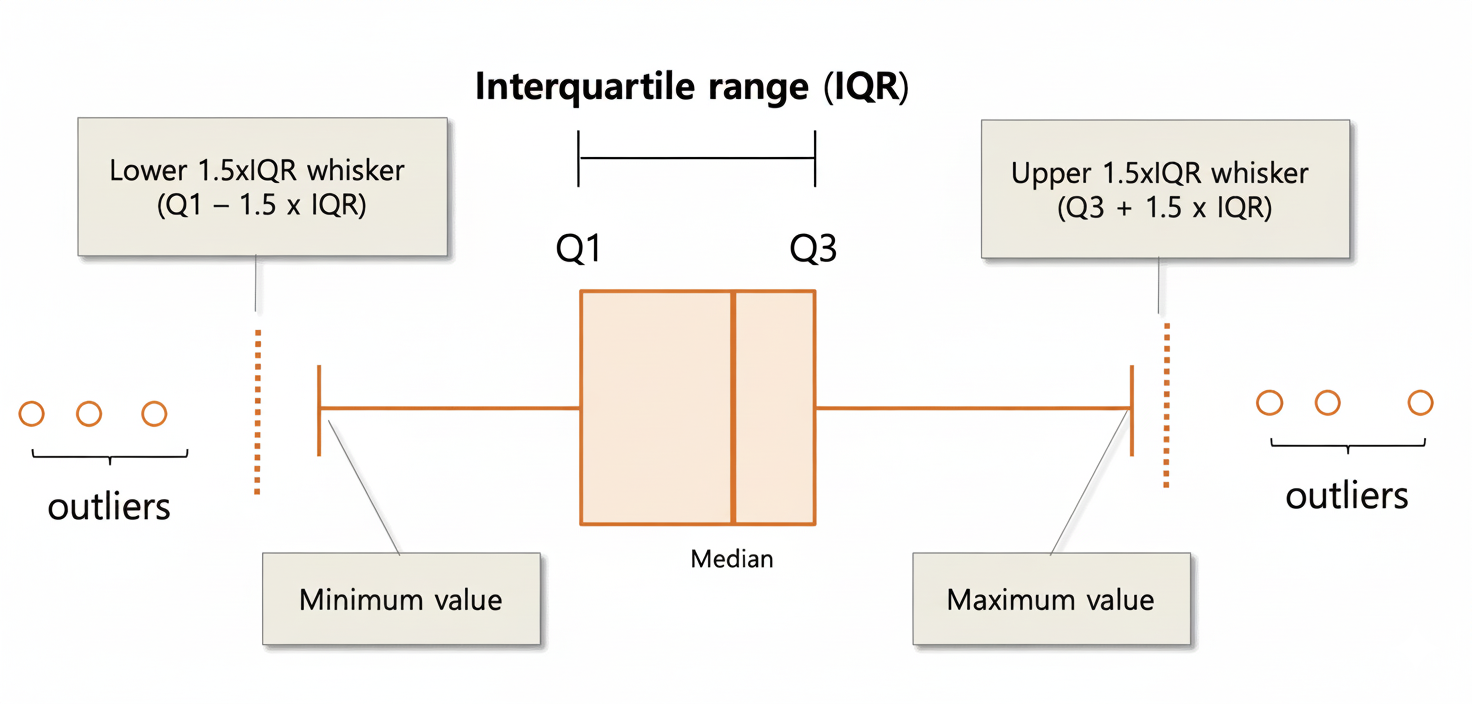
\includegraphics[width=0.7\textwidth]{figure/boxplot.png}
    \caption{An example of a box plot, illustrating the median, quartiles, whiskers, and potential outliers.}
    \label{fig:boxplot_from_image}
\end{figure}


\begin{definition}[Box Plot Components]
A box plot displays five key statistics:
\begin{itemize}
    \item \textbf{Minimum}: The smallest value (excluding outliers)
    \item \textbf{Q1 (First Quartile)}: 25\% of data below this value
    \item \textbf{Median (Q2)}: 50\% of data below this value
    \item \textbf{Q3 (Third Quartile)}: 75\% of data below this value
    \item \textbf{Maximum}: The largest value (excluding outliers)
    \item \textbf{Outliers}: Points beyond 1.5 × IQR from the box
\end{itemize}
\end{definition}

A box plot provides a visual summary of the distribution of a dataset, making it easy to compare groups and spot outliers. Here's how to read a box plot.

\begin{itemize}
    \item The \textbf{length of the box} shows the spread of the central half of the data. A longer box means more variability in the middle 50\%.
    \item The \textbf{position of the median line} within the box indicates skewness. If the median is closer to $Q_1$ of the box, the data are skewed right; if closer to $Q_3$ of the box, skewed left.
    \item The \textbf{position of the mean} can be determined by the position of the median line. If the median line is closer to $Q_1$ of the box, the mean is to the left of the median; if closer to $Q_3$ of the box, the mean is to the right of the median.
    \item The \textbf{position of the mode} can also be determined by the position of the median line. If the median line is closer to $Q_1$ of the box, the mode is to the left of the median; if closer to $Q_3$ of the box, the mode is to the right of the median.
    \item The \textbf{whiskers} show the range of the bulk of the data, excluding outliers.
    \item \textbf{Outliers} highlight unusually high or low values that may warrant further investigation.
\end{itemize}

Box plots are especially useful for comparing distributions across several groups or datasets, as they quickly reveal differences in medians, spreads, and the presence of outliers.

This concludes our discussion of data visualization and summary statistics, and in general our discussion of probability and statistics.